\documentclass[11pt, reqno, letterpaper, twoside]{amsart}
\linespread{1.2}
\usepackage[margin=1.25in]{geometry}

\usepackage{listings}
\usepackage{xcolor}

\lstset{
    language=Python,
    basicstyle=\ttfamily\small,
    keywordstyle=\color{blue},
    stringstyle=\color{red},
    commentstyle=\color{green!50!black},
    numbers=left,
    numberstyle=\tiny,
    stepnumber=1,
    numbersep=5pt,
    showstringspaces=false,
    breaklines=true,
    frame=single,
}

\usepackage{pythonhighlight}
\usepackage{amssymb, bm, mathtools,physics}
\usepackage[usenames,dvipsnames,svgnames,table]{xcolor}
\usepackage[pdftex, xetex]{graphicx}
\usepackage{enumerate, setspace}
\usepackage{float, colortbl, tabularx, longtable, multirow, subcaption, environ, wrapfig, textcomp, booktabs}
\usepackage{pgf, tikz, framed}
\usepackage[normalem]{ulem}
\usetikzlibrary{arrows,positioning,automata,shadows,fit,shapes}
\usepackage[english]{babel}

\usepackage[final]{microtype}

\theoremstyle{plain}
\newtheorem{theorem}{Theorem}

\theoremstyle{definition}
\newtheorem{solution}[theorem]{Solution}
\renewcommand{\solution}{\textbf{Solution}\newline}


\usepackage{times}
\title{ESE 546\\[0.1in]
Homework 1}
\author{
Ravi Raghavan [rr1133@seas.upenn.edu],\\
Collaborators: N/A
}

\begin{document}
\maketitle

% Important LInks
% 1. https://scikit-learn.org/stable/modules/svm.html#implementation-details
% 2. https://scikit-learn.org/stable/auto_examples/svm/plot_svm_kernels.html#sphx-glr-auto-examples-svm-plot-svm-kernels-py
% 3. https://www.csie.ntu.edu.tw/~cjlin/papers/libsvm.pdf
% 4. https://scikit-learn.org/stable/auto_examples/svm/plot_rbf_parameters.html

% https://scikit-learn.org/stable/modules/svm.html#svm-mathematical-formulation
\begin{solution}[Time spent: 1 hour]
\begin{enumerate}
    \item[(a)] The slack-variable based optimization problem can be formulated as such
    \begin{align}
        \label{eq:1a-1}
            \begin{array}{ll}
\text{minimize}_{\theta, \theta_0, \xi_1, \cdots, \xi_n} & \frac{1}{2} \|\theta\|^2 +  C \sum_{i = 1}^n \xi_i \\
\text{subject to} & y_i (\theta^T x_i + \theta_0) \geq 1 - \xi_i,\, \forall i = 1, \cdots, n \\
& \xi_i \geq 0,\, \forall i = 1, \cdots, n
\end{array}
        \end{align}

    where $C$ is a hyperparameter and our optimization variables are $\theta, \theta_0, \xi_1, \cdots, \xi_n$. \\
    \noindent From \eqref{eq:1a-1}, we observe that a larger value of $C$ places a stronger penalty on slack, reducing the margin and prioritizing correct classification of training points. Conversely, a smaller value of $C$ allows more slack, resulting in a wider margin and greater tolerance for misclassifications.  

\textbf{\underline{Answer:}} The objective function is $\frac{1}{2} \|\theta\|^2 +  C \sum_{i = 1}^n \xi_i$, where $C$ is a hyperparameter as described above

    \item[(b)] In an SVM, the support samples are the \textbf{\underline{critical}} data points that determine the position/orientation of the separating hyperplane. Removing any non-support sample would NOT affect the decision boundary. In a Hard-Margin SVM, support samples are samples that lie exactly on the margin boundaries. Mathematically, in the Hard Margin case, we can say that for any given support sample $(x_s, y_s)$, the following holds true 
    \begin{align}
    \label{eq:1a-2}
        y_s (\theta^T x_s + \theta_0) = 1
    \end{align}

    % https://kuleshov-group.github.io/aml-book/contents/lecture13-svm-dual.html#the-dual-of-the-svm-problem
    % https://machine-learning-upenn.github.io/assets/notes/Lec8.pdf
    % https://www.cs.cmu.edu/~aarti/Class/10701_Spring21/Lecs/svm_dual_kernel_inked.pdf

    % https://chatgpt.com/c/68bb1aad-1140-832b-918c-fa8c29b1b32d
    % https://www.csie.ntu.edu.tw/~cjlin/papers/libsvm.pdf
    \noindent In the Soft Margin case, support samples can lie on the margin, within the margin boundaries, or even be a misclassified point. 
    \item[(c)] Check Code
    
    %C-SVM:https://www.csie.ntu.edu.tw/~cjlin/papers/libsvm.pdf
    % C-Parameter: 
    % - https://eitca.org/artificial-intelligence/eitc-ai-mlp-machine-learning-with-python/support-vector-machine/svm-parameters/examination-review-svm-parameters/what-is-the-purpose-of-the-c-parameter-in-svm-how-does-a-smaller-value-of-c-affect-the-margin-and-misclassifications/
    % - https://scikit-learn.org/stable/modules/svm.html#kernel-functions
    % - https://scikit-learn.org/stable/auto_examples/svm/plot_rbf_parameters.html#sphx-glr-auto-examples-svm-plot-rbf-parameters-py
    \item[(d)] $C$ is a regularization parameter that controls the tradeoff between correctly classifying training points and maximizing the margin. A larger $C$ strongly penalizes misclassified points, favoring correct classification even if it results in a narrower margin. This can reduce generalization, making the model more sensitive to the training data. Conversely, a smaller $C$ tolerates some misclassifications, resulting in a wider margin and even better generalization. \\

    \noindent $\gamma$ is the kernel coefficient in rbf, polynomial, and sigmoid kernels, determining the reach of each training point's influence. This influence refers to a region around a training point where the kernel function assigns significant weight when computing similarities. A small $\gamma$ gives each training data point a broad influence, producing a smoother, more generalized decision boundary and better overall generalization. On the other hand, a larger $\gamma$ restricts each point's influence to a narrow area, enabling the model to fit the training data closely, which can increase overfitting and reduce generalization. \\  

    In Scikit-learn, the default value of $C$ is $1.0$, and the default value of $\gamma$ is "scale", which is computed as $\frac{1}{n_{\text{features}} * X.var()}$, where $n_{\text{features}}$ is the number of features and $X.var()$ is the variance of all the values in the design matrix. \\

    When running the given SVM Classifier, here are the experimental results \\
    \textbf{Experimental Results:}
    \begin{itemize}
        \item Training Accuracy: 
        \item Training Error: 
        \item Validation Accuracy: 
        \item Validation Error: 
        \item Support Vector Ratio: 
        \item Test Accuracy: 
        \item Test Error: 
    \end{itemize}

    % \begin{figure}[h!]
    %     \centering
    %     \includegraphics[width=0.5\linewidth]{confusion_matrix_1d.png}
    %     \caption{Confusion Matrix}
    %     \label{fig:placeholder}
    % \end{figure}

% \textbf{Identifying the Pattern:} \\
% From the confusion matrix, we can see that the SVM classifier predicts only $9$ for all test samples, which is the clear pattern here.  \\

% \textbf{Intuitive Explanation: } \\
% To understand this behavior, we examine the classifier's hyperparameters, starting with $\gamma$. By default, $\gamma = \tfrac{1}{n_{\text{features}} \cdot X.var()}$, but in our case we set $\gamma = \text{auto}$, which instead uses $\gamma = \tfrac{1}{n_{\text{features}}}$. For our dataset, $X.var() \approx 5164$, so choosing $\gamma = \text{auto}$ made our $\gamma$ value about $5164$ times larger than the default. From our earlier discussion, we know that having a higher $\gamma$ value restricts each point's influence to a narrow area, enabling the model to fit the training data closely, which can increase overfitting and reduce generalization. \\

\noindent \textbf{Extra: Improving Performance by Tweaking $\gamma$ to $\text{scale}$} \\
\textbf{Experimental Results:}
    \begin{itemize}
        \item Training Accuracy: 
        \item Training Error: 
        \item Validation Accuracy: 
        \item Validation Error: 
        \item Support Vector Ratio: 
        \item Test Accuracy: 
        \item Test Error: 
    \end{itemize}

% \begin{figure}[h!]
%     \centering
%     \includegraphics[width=0.5\linewidth]{confusion_matrix_1d_2.png}
%     \caption{Confusion Matrix}
%     \label{fig:placeholder}
% \end{figure}

\item[(e)] We will list out the parameters from Scikit-learn and analyze each of them: 
\begin{itemize}
    \item C: Already discussed previously
    \item kernel: Kernel function to use 
    \item degree: the degree of the polynomial kernel 
    \item gamma: Already discussed previously
    \item coef0: Independent term in polynomial and sigmoid kernels
    \item shrinking: 
    \item probability: 
    \item tol:
    \item $\text{cache\_size}$: Size of kernel cache in MB
    \item verbose: 
    \item $\text{max\_iter}$
    \item $\text{decision\_function\_shape}$
    \item $\text{break\_ties}$
    \item $\text{random\_state}$: 

\end{itemize}
    
\end{enumerate}
\end{solution}

\clearpage
% https://stanford.edu/class/ee364b/lectures/subgradients_notes.pdf
% https://stanford.edu/class/ee364b/lectures/subgradients_slides.pdf
\begin{solution}[Time spent: 10 minutes] \\
In what follows, we establish Jensen’s Inequality in the more general setting where $X$ can take values in an infinite set. As per the problem statement, we subsequently assume that $\varphi$ is differentiable \\

\noindent Denote \( g = \nabla \varphi(\mu) \).  
By the first-order characterization of convexity, we have
\[
\varphi(x)\geq \varphi(\mu) + g^\top (x - \mu), 
\quad \forall x \in \mathbb{R}^n.
\]

Applying the above inequality to the random vector \(X\) gives us the following
\[
\varphi(X)\ge \varphi(\mu)+ g^\top \left(X-\mu\right)
\]

%https://imai.fas.harvard.edu/teaching/files/Expectation.pdf
Taking Expectation of both sides of the inequality gives us 
\[
\mathbf{E} \left[ \varphi(X) \right]\ge \mathbf{E} \left[ \varphi(\mu)+ g^\top \left(X-\mu\right) \right]
\]

Using Linearity of Expectation, we see that
\[
\mathbf{E} \left[ \varphi(X) \right]\ge \mathbf{E} \left[ \varphi(\mu) \right] + \mathbf{E} \left[ g^\top \left(X-\mu\right) \right]
\]

We use Linearity of Expectation on $\mathbf{E} \left[ g^\top \left(X-\mu\right) \right]$ to further simplify
\[
\mathbf{E} \left[ \varphi(X) \right]\ge \mathbf{E} \left[ \varphi(\mu) \right] + g^\top \cdot \mathbf{E} \left[\left(X-\mu\right) \right]
\]

Using Linearity of Expectation on $\mathbf{E} \left[\left(X-\mu\right) \right]$, we simplify 
\[
\mathbf{E} \left[ \varphi(X) \right]\ge \mathbf{E} \left[ \varphi(\mu) \right] + g^\top \cdot \left( \mathbf{E} \left[X \right] - \mathbf{E} \left[\mu \right] \right)
\]

Finally, we use the fact that $\varphi(\mu)$ and $\mu$ are deterministic and that \(\mathbb{E}[X]=\mu\) to simplify
\[
\mathbf{E} \left[ \varphi(X) \right]\ge \varphi(\mu) + g^\top \cdot \left( \mu - \mu \right)
\]
\[
\mathbf{E} \left[ \varphi(X) \right]\ge \varphi(\mu) + g^\top \cdot \left( 0 \right)
\]
\[
\mathbf{E} \left[ \varphi(X) \right]\ge \varphi(\mu)
\]

This proves the claimed inequality.

\end{solution}

\clearpage
\begin{solution}[Time spent: 1 hour]
\begin{enumerate}
    \item[(a)] 
    \textit{Note: At the start of this problem, I set the random seed to 42 to ensure consistent and reproducible results.} 
    \begin{python}
# Throughout the entire problem, I set the random state here for reproducability
random_state = 42
    \end{python}

Once the random seed was set, I downloaded the MNIST dataset using the following code 
\begin{python}
### Load Data from torchvision using the Code provided by the assignment
import torchvision as thv
train = thv.datasets.MNIST("./", download=True, train=True)
val = thv.datasets.MNIST("./", download=True, train=False)
print("Part (a): Print out shape of train.data, train.targets, val.data, and val.targets")
print(train.data.shape, len(train.targets), val.data.shape, len(val.targets))

\end{python}

As expected, from my print statements, the training data had $60000$ samples where each image was $28 \times 28$. The validation data had $10000$ samples where each image was $28 \times 28$. Both training and validation targets were spread across 10 classes. After loading the data, I converted everything to NumPy arrays. Following the problem instructions, all neural network implementation is done using only NumPy and basic Python. Attached below is the corresponding code
\begin{python}
### Convert the above PyTorch Tensors to numpy. From here on out, NO Torch/Other Deep Learning Library 
### PyTorch will ONLY be used at the VERY END to verify my results
import numpy as np
np.random.seed(random_state) # set random state, throughout the entire problem, for reproducability
X_train = train.data.numpy()
y_train = train.targets.numpy()
X_val = val.data.numpy()
y_val = val.targets.numpy()
print("Part (a): Print out shape of X_train, y_train, X_val, and y_val after converting to numpy")
print(X_train.shape, y_train.shape, X_val.shape, y_val.shape)
\end{python}

Next, I normalized the MNIST data from [0, 255] to [0, 1] to improve training stability for the neural network. Attached below is the corresponding code 
\begin{python}
    ### Normalize Data
X_train = X_train.astype(np.float64) / 255.0
X_val = X_val.astype(np.float64) / 255.0
\end{python}

Finally, to create my dataset, I took $50\%$ of the images from each class for training and validation, i.e., about 30,000 training images and 5,000 validation images, almost evenly spread across all classes, with a few minor differences. Attached below is the corresponding code 
\begin{python}
    ### Given X and y, where X contains training samples and y contains labels, keep only 50% of each class! 
def downsample(X, y):
    # Store downsampled X and y
    X_downsampled, y_downsampled = [], []

    # Iterate through the unique labels of y
    for label in np.unique(y):
        indices = np.where(y == label)[0] # Fetch indices where y == label
        indices = np.sort(indices)
        half = len(indices) // 2 # Get half
        X_downsampled.append(X[indices[:half]])
        y_downsampled.append(y[indices[:half]])
    
    return np.concatenate(X_downsampled, axis = 0), np.concatenate(y_downsampled, axis = 0)

### Perform downsampling on X_train, y_train, X_val, y_val
X_train, y_train = downsample(X_train, y_train)
X_val, y_val = downsample(X_val, y_val)
print("Part (a): Print out shape of X_train, y_train, X_val, and y_val after downsampling")
print(X_train.shape, y_train.shape, X_val.shape, y_val.shape)

\end{python}

Finally, once our data has been loaded, converted to numpy, normalized, and then downsampled, we plot a few images to verify integrity of the data. Attached below is the code used to generate the plots as well as a few sample images from training and validation datasets! 
\begin{python}
    ## Plot the images of a few images in the dataset just to see if label is right
# Function to plot a grid of images with labels
import matplotlib.pyplot as plt
def plot_images_random(X, y, file_title, fig_title=None, n_images=16):
    indices = np.random.choice(len(X), size=n_images, replace=False)
    plt.figure(figsize=(8, 8))

    if fig_title:
        plt.suptitle(fig_title, fontsize=16)

    for i, idx in enumerate(indices):
        plt.subplot(4, 4, i+1)
        plt.imshow(X[idx], cmap='gray')
        plt.title(f"Label: {y[idx]}")
        plt.axis('off')
    plt.tight_layout()
    plt.savefig(file_title, dpi=300)

# Plot first 16 images from the downsampled training set
plot_images_random(X_train, y_train, "3a_train_images.png", "Training Images w/ Labels")
plot_images_random(X_val, y_val, "3a_val_images.png", "Validation Images w/ Labels")

\end{python}

\begin{figure}[h!]
    \centering
    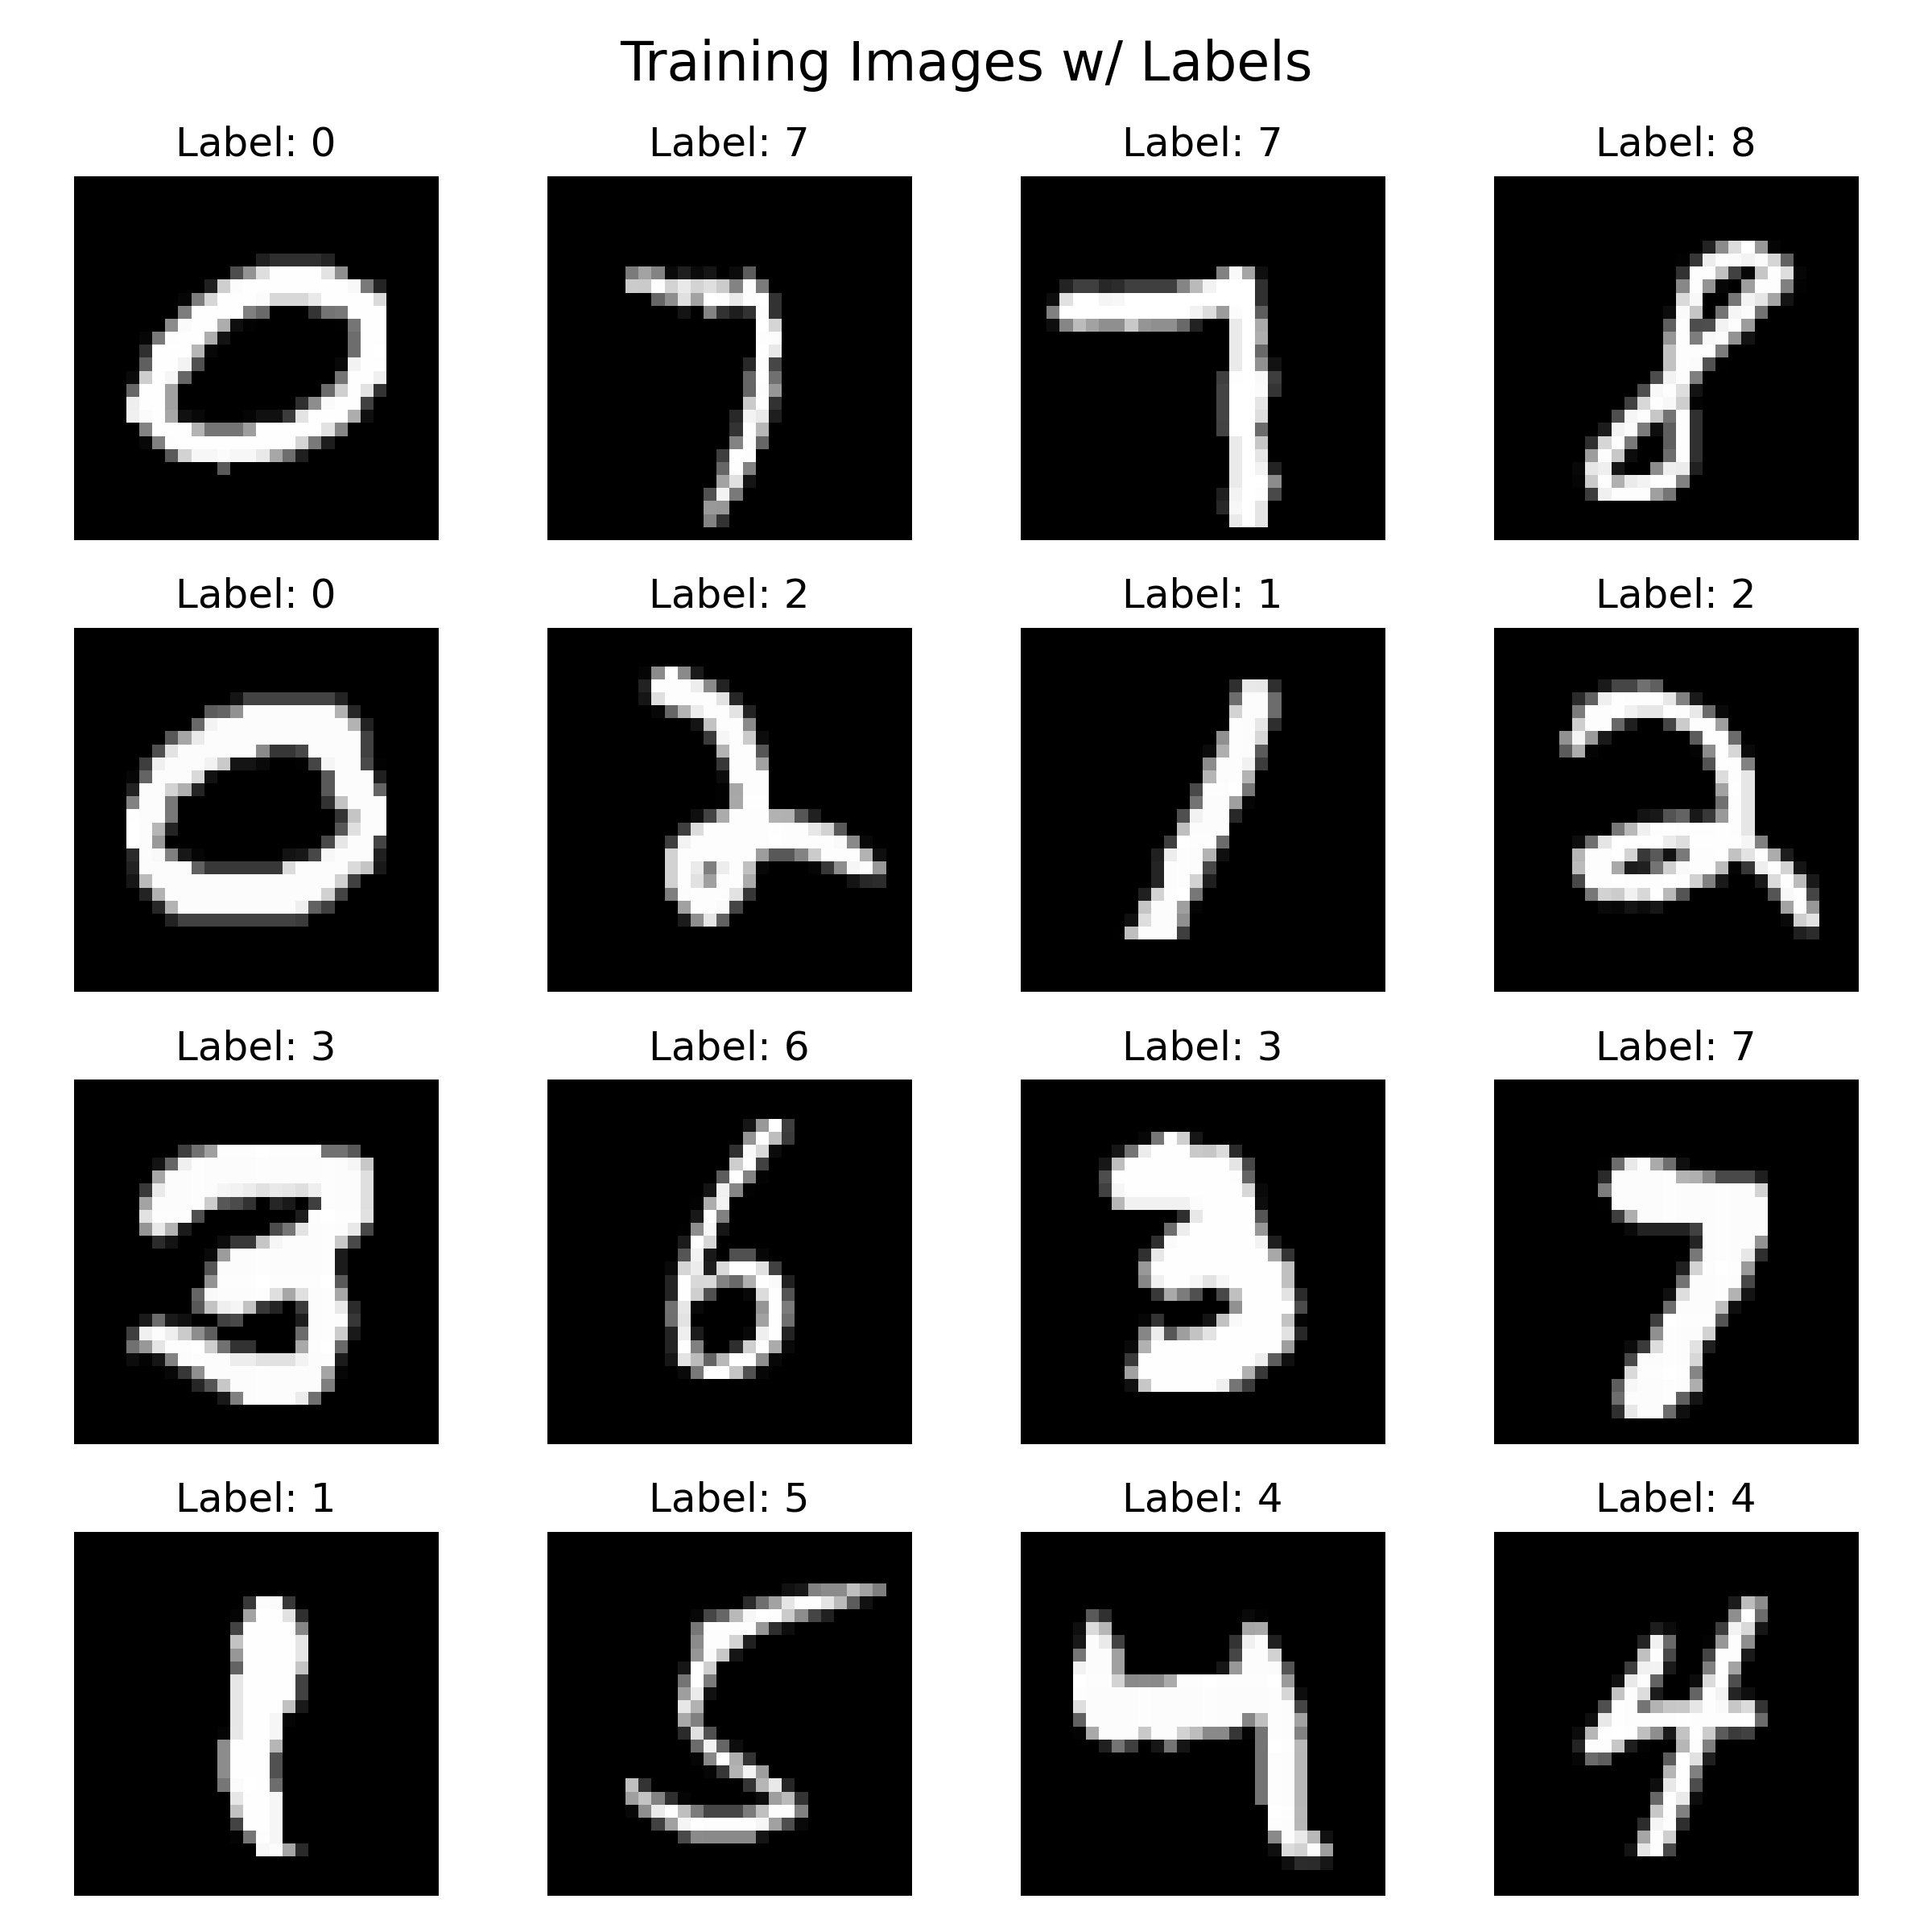
\includegraphics[width=0.4\linewidth]{3a_train_images.png}
    \caption{Training Images with their labels}
    \label{fig:3-a-train-images}
\end{figure}

\begin{figure}[h!]
    \centering
    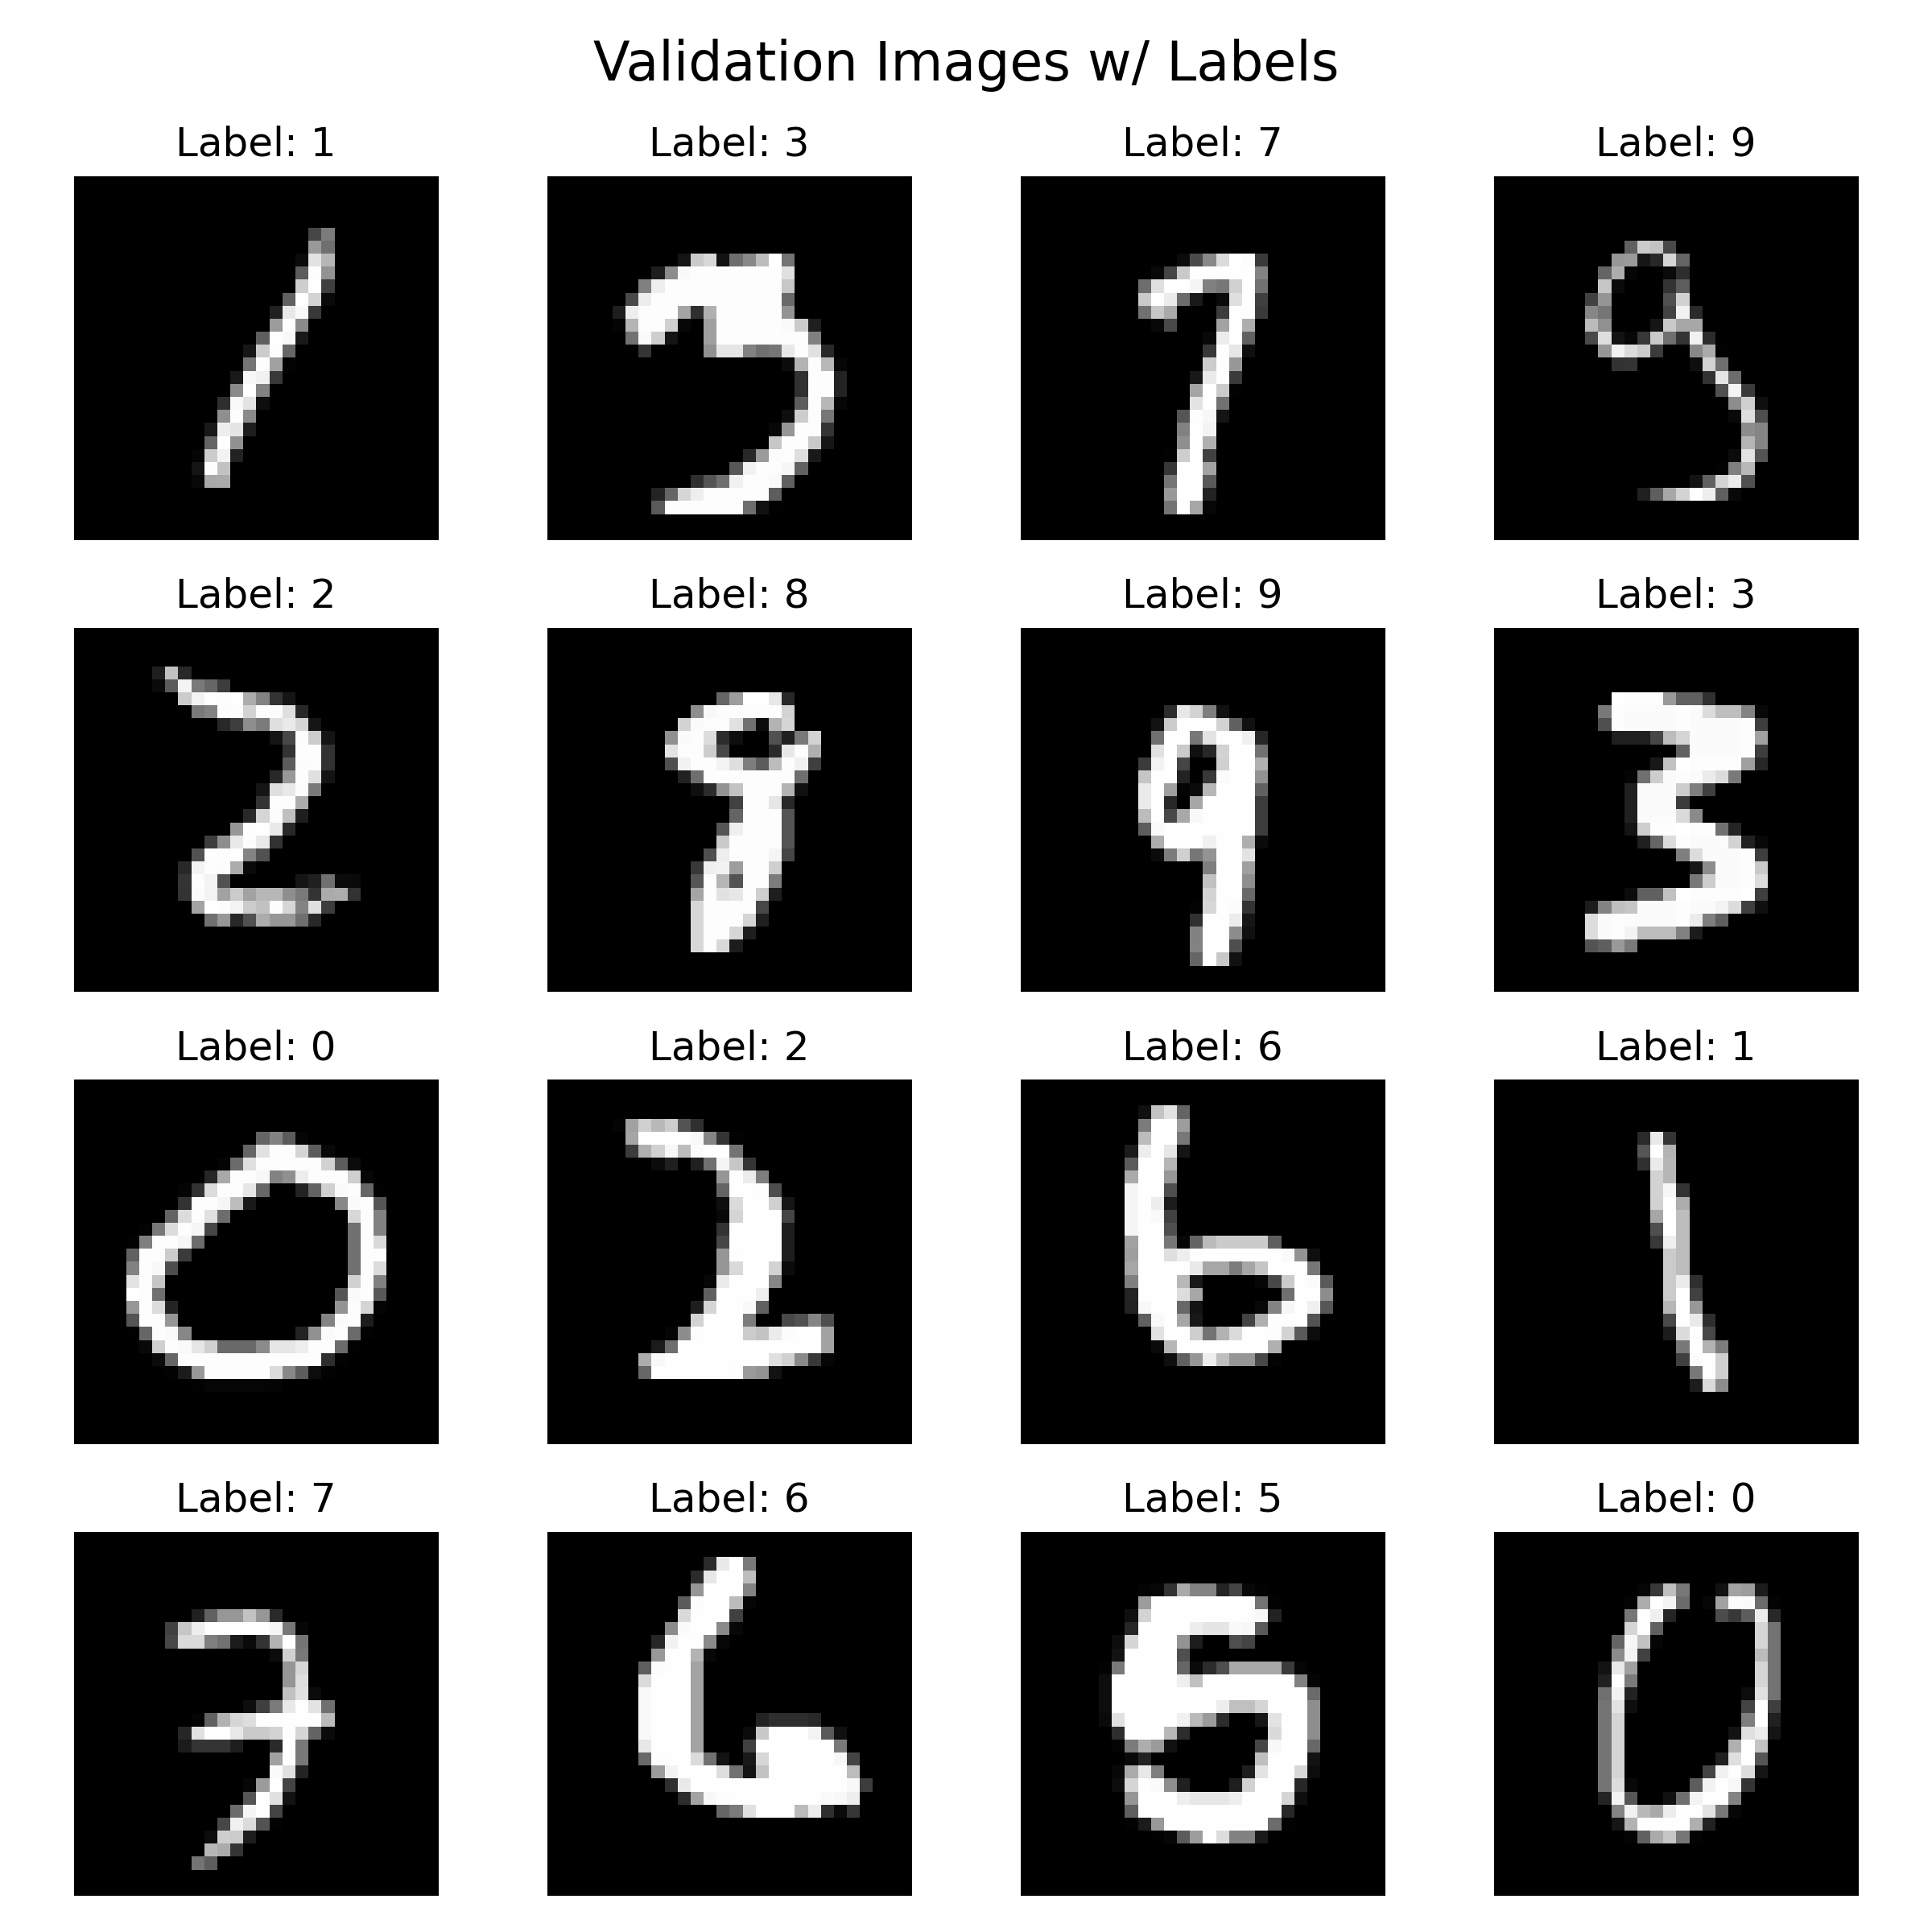
\includegraphics[width=0.4\linewidth]{3a_val_images.png}
    \caption{Validation Images with their labels}
    \label{fig:3-a-val-images}
\end{figure}

\newpage 
\item[(b)] The goal was to implement the embedding layer from the Homework PDF. Below is the code.
\begin{python}
    ## Problem 3, Part (b)
class embedding_t:
    def __init__(self):
        # initialize to appropriate sizes, fill with Gaussian entries
        mean = 0.0
        std = 0.01
        self.w = np.random.normal(loc = mean, scale = std, size = (4, 4, 8))
        self.b = np.random.normal(loc = mean, scale = std, size = (8,))

        # normalize to make the Frobenius norm of (w, b) equal to 1
        fro_norm = np.sqrt(np.sum(self.w ** 2) + np.sum(self.b ** 2))
        self.w = self.w / fro_norm
        self.b = self.b / fro_norm
    
    def zero_grad(self):
        # useful to delete the stored backprop gradients of the previous mini-batch before you start a new mini-batch
        self.dw, self.db = 0, 0

    # Shape of hl: B x 28 x 28
    def forward(self, hl):
        # Store Batch Value
        B = hl.shape[0]

        # We denote dimension of hl as B X 28 X 28 where B is the batch size
        # Step 1: Convert hl to B X 28 X 28 X 1
        hl = hl[:, :, :, None]

        # Step 2: Convert hl to B X 28 X 28 X 8
        hl = np.repeat(hl, repeats = 8, axis = -1)

        # We cache hl in forward because we need to compute it in backward
        self.hl = hl

        # Step 3: Form Sliding Windows: Shape is B x 25 x 25 x 1 x 4 x 4 x 8
        sliding_windows = np.lib.stride_tricks.sliding_window_view(hl, window_shape = (4, 4, 8), axis = (1, 2, 3))
        
        # Step 4: To capture Stride in our convolution, subset windows and we now have B x 7 x 7 x 4 x 4 x 8
        sliding_windows = sliding_windows[:, ::4, ::4, 0]

        # Step 5: Element-wise multiplication to get output of B x 7 x 7 x 8
        hl_plus_1 = (sliding_windows * self.w).sum(axis = (3, 4)) + self.b

        # Step 6: Convert to B x 392
        hl_plus_1 = hl_plus_1.reshape(B, -1)

        return hl_plus_1
    
    # dhl_plus_1 Shape: B x 392
    def backward(self, dhl_plus_1):
        # Store Batch Value
        B = dhl_plus_1.shape[0]

        # Step 1: Reshape as B x 7 x 7 x 8
        dhl_plus_1 = dhl_plus_1.reshape(B, 7, 7, 8)

        # Bring back self.hl and create sliding windows
        # Step 2: Form Sliding Windows: Shape is B x 25 x 25 x 1 x 4 x 4 x 8
        sliding_windows = np.lib.stride_tricks.sliding_window_view(self.hl, window_shape = (4, 4, 8), axis = (1, 2, 3))
        
        # Step 3: To capture Stride in our convolution, subset windows and we now have B x 7 x 7 x 4 x 4 x 8
        sliding_windows = sliding_windows[:, ::4, ::4, 0]

        # Step 4: Compute dw and db
        dhl_plus_1_reshaped = dhl_plus_1[:, :, :, None, None, :] # Reshape to B x 7 x 7 x 1 x 1 x 8
        dw = (sliding_windows * dhl_plus_1_reshaped).sum(axis = (0, 1, 2))
        db = dhl_plus_1_reshaped.sum(axis = (0, 1, 2, 3, 4))

        # Step 5: Store gradients for w and b
        self.dw, self.db = dw, db

        # Step 6: Compute dhl
        dhl = (self.w * dhl_plus_1_reshaped).sum(axis = -1) # B x 7 x 7 x 4 x 4 
        dhl = dhl.transpose(0, 1, 3, 2, 4).reshape(B, 28, 28) # B x 28 x 28
        return dhl
\end{python}
Below, I present my analysis, outlining the reasoning behind my implementation.   \\
\textbf{\underline{Analysis:}} \\
\textbf{Notation and shapes}
\begin{itemize}
  \item Input to the embedding layer: $h^{(l)} \in \mathbb{R}^{B\times 28 \times 28}$, where $B$ is the mini-batch size.
  \item Weight tensor: $W \in \mathbb{R}^{4\times 4 \times 8}$. I denote its entries as $W_{p,q,k}$ with $p,q\in\{0,1,2,3\}$ and $k\in\{0,\dots,7\}$.
  \item Bias vector: $b \in \mathbb{R}^{8}$ with entries $b_k$.
  \item Output of the embedding (before flatten): $h^{(l+1)} \in \mathbb{R}^{B \times 7 \times 7 \times 8}$ and after flattening per image $h^{(l+1)}_{{\rm flat}} \in \mathbb{R}^{B\times 392}$
  \item In the backward pass, $\delta_{b,i,j,k} \equiv \frac{\partial \mathcal{L}}{\partial h^{(l+1)}_{b,i,j,k}}$ denotes the upstream gradient, with $\mathcal{L}$ denoting the loss function. 
\end{itemize}

\noindent \textbf{Initialization / normalization}
The code initializes $W$ and $b$ with Gaussian entries (mean $0$, std $0.01$) and then normalizes them together so that the Frobenius norm of the concatenated parameters equals $1$:
\[
\text{fro\_norm} = \sqrt{\sum_{p,q,k} W_{p,q,k}^2 \;+\; \sum_{k} b_k^2},\qquad
W \leftarrow \frac{W}{\text{fro\_norm}},\quad b \leftarrow \frac{b}{\text{fro\_norm}}.
\]

\noindent \textbf{High-level description}
This embedding layer implements a \emph{2D convolution} with kernel size $4\times 4$, stride $4$, single input channel, and $8$ output channels. Concretely, the image $28\times 28$ is partitioned into non-overlapping $4\times4$ patches (there are $7\times7$ such patches). For each patch the layer computes an $8$-dimensional vector by multiplying each scalar pixel in the patch by a corresponding $8$-dimensional weight vector and summing over the 16 pixels, then adding the bias $b$. This is equivalent to a standard Conv2D with $(\text{out\_channels}=8,\ \text{in\_channels}=1,\ \text{kernel}=4,\ \text{stride}=4)$ \\

\noindent \textbf{Forward Pass}
Let $x_{b,u,v}$ be the pixel at batch index $b$ and coordinates $(u,v)$, where $u,v \in {0,\dots,27}$. By the convolution process, the $28\times28$ image is divided into $4\times4$ patches, producing a $7\times7$ grid indexed by $(i,j)$ with $i,j \in {0,\dots,6}$. The top-left pixel of patch $(i,j)$ lies at $(4i,4j)$ in the global image coordinates, and within the patch, $(p,q)$ denotes the local position, where $p,q \in {0,1,2,3}$. \\

The forward formula for each output channel $k$ is:
\begin{align}
h^{(l+1)}_{b,i,j,k}
&= \sum_{p=0}^{3}\sum_{q=0}^{3} W_{p,q,k}\; x_{b,\,4i+p,\,4j+q} \;+\; b_k.
\label{eq:forward_explicit}
\end{align}

\textit{Note: $h^{(l+1)}_{b,i,j,k}$ \text{ is the value at batch index} $b$, \text{ patch } $(i,j)$, \text{ and output channel } $k$ \text{ in the output layer }.
}

Vectorizing across $k$ gives $h^{(l+1)}_{b,i,j,:}\in\mathbb{R}^8$. After computing \eqref{eq:forward_explicit} for all $(i,j)$ we flatten each $7\times7\times8$ tensor into a $392$-dimensional vector to form the returned array $h^{(l+1)}_{{\rm flat}} \in \mathbb{R}^{B\times 392}$. \\

\paragraph{Forward Pass NumPy Implementation}
\begin{enumerate}
  \item \texttt{hl = hl[:, :, :, None]}: add a channel axis so the input becomes shape $(B,28,28,1)$.
  \item \texttt{hl = np.repeat(hl, repeats=8, axis=-1)}: replicate the scalar pixel value across an 8-length channel axis to produce $\hat h\in\mathbb{R}^{B\times 28\times 28\times 8}$ where $\hat h_{b,u,v,k} = x_{b,u,v}$ for all $k$. This enables the eventual elementwise multiplication of image patches with $W_{p,q,k}$.
  \item \texttt{sliding\_window\_view(..., window\_shape=(4,4,8), axis=(1,2,3))}: this produces all contiguous windows of size $4 \times 4 \times 8$; the result has shape $(B,\,25,\,25,\,1,\,4,\,4,\,8)$ because along axes 1 and 2 there are $28-4+1 = 25$ start positions and along axis 3 (channel axis of length 8) there is exactly one start position for window-size 8.
  \item \texttt{sliding\_windows = sliding\_windows[:, ::4, ::4, 0]}: selecting every 4th starting position implements stride $4$; after this we have $\texttt{sliding\_windows}\in\mathbb{R}^{B\times 7\times 7\times 4\times 4 \times 8}$ where
    \[
    \texttt{sliding\_windows}[b,i,j,p,q,k] = x_{b,\,4i+p,\,4j+q}.
    \]
  \item \texttt{hl\_plus\_1 = (sliding\_windows * self.w).sum(axis=(3,4)) + self.b}: elementwise multiply the window tensor with $W$ and sum over the $4\times4$ patch dims; this realizes \eqref{eq:forward_explicit} for all $(b,i,j,k)$ at once, producing shape $(B,7,7,8)$. Adding \texttt{self.b} broadcasts the bias $b_k$ to each spatial location.
  \item \texttt{hl\_plus\_1 = hl\_plus\_1.reshape(B, -1)}: flatten to $(B,392)$.
\end{enumerate}

\noindent \textbf{Backward Pass }
Let $\delta_{b,i,j,k}=\dfrac{\partial \mathcal{L}}{\partial h^{(l+1)}_{b,i,j,k}}$. Referencing \eqref{eq:forward_explicit}, we see that: 
\begin{align}
\frac{\partial \mathcal{L}}{\partial b_k}
&= \sum_{b=1}^{B}\sum_{i=0}^{6}\sum_{j=0}^{6} \delta_{b,i,j,k}, \label{eq:grad_b}\\[6pt]
\frac{\partial \mathcal{L}}{\partial W_{p,q,k}}
&= \sum_{b=1}^{B}\sum_{i=0}^{6}\sum_{j=0}^{6} \delta_{b,i,j,k} \; x_{b,\,4i+p,\,4j+q}. \label{eq:grad_w}
\end{align}
The input gradient for a pixel $x_{b,u,v}$ where $u=4i+p$, $v=4j+q$, for unique integers $i,j,p,q$ because patches are non-overlappin,  is
\begin{align}
\frac{\partial \mathcal{L}}{\partial x_{b,u,v}}
&= \sum_{k=0}^{7} W_{p,q,k}\; \delta_{b,i,j,k},\qquad\text{with } i=\lfloor u/4\rfloor,\ p = u \bmod 4,\ \text{similarly for } j,q.
\label{eq:grad_x}
\end{align}
Because stride $=4$ and patch size $=4$, each input pixel participates in exactly one patch, so the above indexing is unique and well-defined. \\

\paragraph{Backward Pass NumPy Implementation}
\begin{enumerate}
  \item The upstream gradient \texttt{dhl\_plus\_1} arrives with shape $(B,392)$ and is reshaped to $(B,7,7,8)$ to produce $\delta_{b,i,j,k}$.
  \item \texttt{dhl\_plus\_1\_reshaped = dhl\_plus\_1[:,:,:,None,None,:]} creates $\Delta \in \mathbb{R}^{B\times 7\times 7\times 1\times 1 \times 8}$ which can broadcast against the window tensor.
  \item \texttt{dw = (sliding\_windows * dhl\_plus\_1\_reshaped).sum(axis=(0,1,2))} implements \eqref{eq:grad_w} exactly: multiply every scalar window value $x_{b,4i+p,4j+q}$ by the corresponding $\delta_{b,i,j,k}$ (broadcast along $p,q$), then sum over $b,i,j$ to get a $4\times4\times 8$ tensor.
  \item \texttt{db = dhl\_plus\_1\_reshaped.sum(axis=(0,1,2,3,4))} sums the upstream gradients over batch and spatial locations to implement \eqref{eq:grad_b}.
  \item To compute the input gradient we use the identity in \eqref{eq:grad_x}. \[
    \texttt{dhl} = (W * dhl\_plus\_1\_reshaped).sum(axis=-1)
    \]
    Here \texttt{W} broadcasts to shape $(B,7,7,4,4,8)$ and the sum over axis $-1$ (the 8 channels) yields an array of shape $(B,7,7,4,4)$ whose entry $(b,i,j,p,q)$ equals $\sum_k W_{p,q,k}\,\delta_{b,i,j,k}$.
    Finally the code reorders axes and reshapes:
    \[
    \texttt{dhl} = \texttt{dhl.transpose(0,1,3,2,4).reshape(B,28,28)}
    \]
    which maps the $(i,p,j,q)$ layout to a dense grid of shape $28\times 28$, producing $\partial\mathcal{L}/\partial x$ with the same shape as the input $h^{(l)}$. \\
\end{enumerate}


\noindent \textbf{Summary}
Overall, this layer performs a convolution with a $4 \times 4$ kernel, stride 4, mapping from a single input channel to 8 output channels.

\newpage 

\item[(c)] The goal was to implement the standard linear layer from the Homework PDF. Below is the code
\begin{python}
## Problem 3, Part (c)
class linear_t:
    def __init__(self):
        # initialize to appropriate sizes, fill with Gaussian entries
        mean = 0.0
        std = 0.01
        self.w = np.random.normal(loc = mean, scale = std, size = (10, 392))
        self.b = np.random.normal(loc = mean, scale = std, size = (10,))

        # normalize to make the Frobenius norm of (w, b) equal to 1
        fro_norm = np.sqrt(np.sum(self.w ** 2) + np.sum(self.b ** 2))
        self.w = self.w / (fro_norm)
        self.b = self.b / (fro_norm)
    
    def zero_grad(self):
        # useful to delete the stored backprop gradients of the previous mini-batch before you start a new mini-batch
        self.dw, self.db = 0, 0
    
    def forward(self, hl):
        # Cache hl in forward because needed for back
        self.hl = hl

        # Compute h_{l + 1}
        hl_plus_1 = hl @ self.w.T + self.b

        return hl_plus_1
    
    # Shape of dhl_plus_1: B x 10
    def backward(self, dhl_plus_1):
        # Compute dhl
        dhl = dhl_plus_1 @ self.w
        
        # Compute db
        db = dhl_plus_1.sum(axis = 0)
        self.db = db

        # Compute dw
        dw = dhl_plus_1.T @ self.hl
        self.dw = dw

        return dhl
\end{python}

Below, I present my analysis, outlining the reasoning behind my implementation.   \\
\textbf{\underline{Analysis:}} \\
\textbf{Notation and shapes.}
\begin{itemize}
  \item $B$ : mini-batch size (number of examples in the current batch).
  \item $a$ : input feature dimension (in this assignment $a=392$).
  \item $c$ : output dimension / number of classes (in this assignment $c=10$).
  \item $H^{(l)}\in\mathbb{R}^{B\times a}$ : the mini-batch of input row-vectors to this layer (variable \verb|hl| in code). Each row $h^{(l)}_i\in\mathbb{R}^a$ is the feature vector for sample $i$.
  \item $W\in\mathbb{R}^{c\times a}$ : weight matrix (variable \verb|self.w|). In the code $W$ has shape $(10,392)$.
  \item $b\in\mathbb{R}^{c}$ : bias vector (variable \verb|self.b|). In code $b$ has shape $(10,)$.
  \item $H^{(l+1)}\in\mathbb{R}^{B\times c}$ : output mini-batch after the linear transform.
  \item For backprop we denote $\Delta := \dfrac{\partial\mathcal{L}}{\partial H^{(l+1)}} \in \mathbb{R}^{B\times c}$ (this is \verb|dhl_plus_1| in the code).
\end{itemize}

\textbf{Initialization and normalization.}
The code draws entries from $\mathcal{N}(0,\sigma^2)$ with $\sigma=0.01$:
\[
W_{jk}\sim\mathcal{N}(0,\sigma^2),\qquad b_j\sim\mathcal{N}(0,\sigma^2).
\]
Then the code computes the combined Frobenius norm of $(W,b)$ and rescales so that the combined norm is $1$: 
\[
\text{fro\_norm}=\sqrt{\sum_{j,k}W_{jk}^2+\sum_j b_j^2},\qquad
W\leftarrow \frac{W}{\text{fro\_norm}},\quad
b\leftarrow\frac{b}{\text{fro\_norm}}.
\]

\textbf{Forward Pass}
The forward computation implemented is the standard affine map applied row-wise to the mini-batch:
\[
H^{(l+1)} = H^{(l)} W^\top + \mathbf{1}_B\, b^\top,
\]
where $\mathbf{1}_B\in\mathbb{R}^{B}$ is the all-ones column vector used conceptually to indicate that $b$ is added to every row (in NumPy the addition uses broadcasting). Equivalently, for each example $i$ (row):
\[
h^{(l+1)}_i = W\, h^{(l)}_i + b \in\mathbb{R}^c.
\]

Code line that implements this:
\begin{verbatim}
hl_plus_1 = hl @ self.w.T + self.b
\end{verbatim}
The code also caches the input batch \verb|self.hl = hl| because it is required to compute the weight gradients in the backward pass.  \\

\textbf{Backward Pass}
Let $\Delta=\dfrac{\partial\mathcal{L}}{\partial H^{(l+1)}}\in\mathbb{R}^{B\times c}$.
We want:
\[
\frac{\partial\mathcal{L}}{\partial H^{(l)}},\qquad
\frac{\partial\mathcal{L}}{\partial W},\qquad
\frac{\partial\mathcal{L}}{\partial b}.
\]

\textbf{$\frac{\partial\mathcal{L}}{\partial H^{(l)}}$: }
Using the forward formula $H^{(l+1)}=H^{(l)}W^\top+b^\top$, the Jacobian of $H^{(l+1)}$ with respect to $H^{(l)}$ is right-multiplication by $W^\top$ so the chain rule gives
\[
\frac{\partial\mathcal{L}}{\partial H^{(l)}} = \Delta\, W \in\mathbb{R}^{B\times a}.
\]
Code:
\begin{verbatim}
dhl = dhl_plus_1 @ self.w
\end{verbatim}

\textbf{$\frac{\partial\mathcal{L}}{\partial b}$:}
Since $b$ is added to every row, the gradient of the loss w.r.t.\ $b$ is the row-wise sum of $\Delta$:
\[
\frac{\partial\mathcal{L}}{\partial b} = \sum_{i=1}^B \Delta_{i,:} \in\mathbb{R}^c.
\]
Code:
\begin{verbatim}
db = dhl_plus_1.sum(axis=0)
self.db = db
\end{verbatim}

\textbf{$\frac{\partial\mathcal{L}}{\partial W}$: }
Consider an element $W_{jk}$ (row $j$, column $k$ of $W$). The contribution to $h^{(l+1)}_{i,j}$ is $W_{j,:}\cdot h^{(l)}_{i,:}$ and therefore
\[
\frac{\partial \mathcal{L}}{\partial W_{jk}} = \sum_{i=1}^{B} \Delta_{i,j}\, h^{(l)}_{i,k}.
\]
In matrix form this becomes
\[
\frac{\partial\mathcal{L}}{\partial W} = \Delta^\top H^{(l)} \in\mathbb{R}^{c\times a}.
\]
Code:
\begin{verbatim}
dw = dhl_plus_1.T @ self.hl
self.dw = dw
\end{verbatim}

\item[(d)] The goal was to implement the ReLU from the Homework PDF. Below is the code
\begin{python}
    ## Problem 3, part (d)
class relu_t:
    def __init__(self):
        pass
    def zero_grad(self):
        pass
    def forward(self, hl):
        # Cache hl in forward because needed for back
        self.hl = hl

        # Compute h_{l + 1}
        hl_plus_1 = np.maximum(0, hl)

        return hl_plus_1
    
    def backward(self, dhl_plus_1):
        return np.where(self.hl < 0, 0, dhl_plus_1)
\end{python}

\noindent \textbf{\underline{Analysis}} \\
\textbf{Notation.}
\begin{itemize}
  \item Let $h^{(l)}\in\mathbb{R}^{B \times d}$ denote the input to the ReLU layer where $B$ is the batch size and $d$ is the dimension of each sample
  \item Let $h^{(l+1)}\in\mathbb{R}^{B \times d}$ denote the output of the ReLU layer where $B$ is the batch size and $d$ is the dimension of each sample
  \item Let $\mathcal{L}$ be the scalar loss; denote
    \[
      \delta^{(l+1)} \equiv \frac{\partial \mathcal{L}}{\partial h^{(l+1)}}
      \qquad\text{and}\qquad
      \delta^{(l)} \equiv \frac{\partial \mathcal{L}}{\partial h^{(l)}}.
    \]
  \item The operator $\odot$ denotes element-wise (Hadamard) multiplication. The indicator function $\mathbf{1}_{\{\cdot\}}$ is $1$ when its condition is true and $0$ otherwise. \\
\end{itemize}

\noindent \textbf{Forward Pass} \\
ReLU is applied element-wise:
\[
  h^{(l+1)}_i \;=\; \max(0,\, h^{(l)}_i), \qquad i=1,\dots,d,
\]
or in vector form
\[
  h^{(l+1)} = \max(0, h^{(l)}),
\]
where the $\max$ is taken element-wise.

In the implementation we cache the input $h^{(l)}$ (stored as \texttt{self.hl}) because the backward pass uses it to construct the derivative mask. \\

\noindent \textbf{Backward Pass} \\
Differentiate each output element with respect to the corresponding input element. For a single element:
\[
  \frac{\partial h^{(l+1)}_i}{\partial h^{(l)}_i}
  \;=\;
  \begin{cases}
    1, & h^{(l)}_i > 0,\\[4pt]
    \text{undefined (subgradient)}, & h^{(l)}_i = 0,\\[4pt]
    0, & h^{(l)}_i < 0.
  \end{cases}
\]
A convenient implementation uses an indicator-mask. In vector form we define the mask
\[
  m \;=\; \mathbf{1}_{\{h^{(l)} \ge 0\}} \in\{0,1\}^{n},
\]
Using this mask, the chain rule gives
\[
  \delta^{(l)} \;=\; \delta^{(l+1)} \odot m.
\]
Expanded elementwise:
\[
  \delta^{(l)}_i = \delta^{(l+1)}_i \cdot \mathbf{1}_{\{h^{(l)}_i \ge 0\}}.
\]

\newpage 

\item[(e)] The goal was to implement the combined softmax and cross-entropy loss layer from the Homework PDF. Below is the code 
\begin{python}
    ## Problem 3, part (e)
class softmax_cross_entropy_t:
    def __init__(self):
        pass

    def zero_grad(self):
        pass

    def forward(self, hl, y):
        # Cache hl in forward because needed for back
        self.hl = hl

        # Flatten y as sanity check 
        y = y.flatten()
        self.y = y

        # Step 1: Compute hl_plus_1 after Softmax
        exp_hl = np.exp(hl)
        hl_plus_1 = exp_hl / np.sum(exp_hl, axis = 1, keepdims=True)

        self.hl_plus_1 = hl_plus_1
        
        # Step 2: Compute average loss over minibatch 
        B = hl.shape[0]

        # Pick the probabilities corresponding to correct labels
        correct_probs = hl_plus_1[np.arange(B), y]
        ell = -np.mean(np.log(correct_probs + 1e-12)) #Adding 1e-12 for numerical stability

        # Step 3: Compute classification error 
        y_pred = np.argmax(hl_plus_1, axis=1)
        error = np.mean(y_pred != y)

        return ell, error

    def backward(self):
        B = self.hl.shape[0]

        # Get output from softmax
        softmax_output = self.hl_plus_1

        # Create one hot labels
        y_one_hot = np.zeros_like(softmax_output)
        y_one_hot[np.arange(B), self.y] = 1

        dhl = (softmax_output - y_one_hot) / B
        return dhl
\end{python}

\textbf{\underline{Analysis}} \\
\textbf{Notation and shapes.}
Let $B$ be the mini-batch size and $C$ the number of classes.  
The layer input (the \emph{logits}) is
\[
h^{(\ell)} \in \mathbb{R}^{B\times C}, \qquad
h^{(\ell)}_{i,k} \text{ is the logit for example } i \text{ and class } k .
\]
The label vector is $y\in\{0,1,\ldots,C-1\}^B$ with $y_i$ the ground-truth class index for example $i$. I denote by $\hat P=\text{softmax}(h^{(\ell)})\in\mathbb{R}^{B\times C}$ the class probabilities with entries $\hat p_{i,k}$. \\

\textbf{Forward Pass}
The implementation follows the definition of the softmax followed by the average cross-entropy loss over the mini-batch.

\begin{enumerate}
\item \textbf{Cache inputs.}
The tensors \verb|hl| (the logits $h^{(\ell)}$) and \verb|y| (the labels) are cached for use in backprop:
\[
\texttt{self.hl} \leftarrow h^{(\ell)}, \qquad \texttt{self.y} \leftarrow y .
\]

\item \textbf{Softmax probabilities.}
\[
\hat p_{i,k}
= \frac{\exp\!\big(h^{(\ell)}_{i,k}\big)}{\sum_{j=1}^C \exp\!\big(h^{(\ell)}_{i,j}\big)}
\quad\Longleftrightarrow\quad
\texttt{hl\_plus\_1 = exp\_hl / sum(exp\_hl, axis=1, keepdims=True)} .
\]
This yields $\hat P\in\mathbb{R}^{B\times C}$ and is stored as \verb|self.hl_plus_1| for the backward pass.

\item \textbf{Average cross-entropy loss.}
For each example, the negative log-probability of the correct class is
\[
\ell_i = -\log \hat p_{i,y_i}.
\]
The following code collects the correct-class probabilities:\\
\texttt{correct\_probs = hl\_plus\_1[np.arange(B), y]}

The following code returns the mean loss
\begin{python}
ell = -np.mean(np.log(correct_probs + 1e-12)) #Adding 1e-12 for numerical stability
\end{python}
 and returns the mean loss
\[
\ell = \frac{1}{B}\sum_{i=1}^B \ell_i
= -\frac{1}{B}\sum_{i=1}^B \log \hat p_{i,y_i}.
\]
\texttt{Note: A small $\varepsilon=10^{-12}$ is added inside the log for numerical safety, 
\(
\log(\hat p_{i,y_i}+\varepsilon)
\), 
to avoid $\log(0)$ when probabilities underflow.}

\item \textbf{Classification error (not part of the loss).}
The predicted class $\hat y_i=\arg\max_k \hat p_{i,k}$ is computed by
\verb|np.argmax(hl_plus_1, axis=1)|.  
The code returns the fraction of misclassified examples,
\[
\mathrm{err}=\frac{1}{B}\sum_{i=1}^B \mathbf{1}\{\hat y_i \neq y_i\}.
\]
\end{enumerate}

\textbf{Backward Pass}
This layer has no learnable parameters, so the gradient to compute is
$\displaystyle \frac{\partial \ell}{\partial h^{(\ell)}} \in \mathbb{R}^{B\times C}$, i.e., the gradient w.r.t. the logits passed to the previous layer.  \\

\underline{Derivation} \\
\indent Write the loss explicitly in terms of the logits:
\[
\ell
= -\frac{1}{B}\sum_{i=1}^B \log
\frac{\exp(h^{(\ell)}_{i,y_i})}{\sum_{j=1}^C \exp(h^{(\ell)}_{i,j})}
= -\frac{1}{B}\sum_{i=1}^B \Big(h^{(\ell)}_{i,y_i} - \log\sum_{j=1}^C \exp(h^{(\ell)}_{i,j})\Big).
\]

\indent Differentiate w.r.t. a particular logit $h^{(\ell)}_{i,k}$:
\[
\frac{\partial \ell}{\partial h^{(\ell)}_{i,k}}
= -\frac{1}{B}\,\mathbf{1}\{k=y_i\}
+\frac{1}{B}\,\frac{\exp(h^{(\ell)}_{i,k})}{\sum_{j=1}^C \exp(h^{(\ell)}_{i,j})}
= \frac{1}{B}\Big(\hat p_{i,k}-\mathbf{1}\{k=y_i\}\Big).
\]
In matrix form, with $Y\in\{0,1\}^{B\times C}$ the one-hot encoding of the labels ($Y_{i,k}=\mathbf{1}\{k=y_i\}$),
\[
\nabla_{h^{(\ell)}} \ell
= \frac{1}{B}\big(\hat P - Y\big).
\]

\item[(f)]

\textbf{\underline{Embedding Layer}} \\
Here is the code I used to check whether the Backward Pass was working for the Embedding Layer
\begin{python}
    ### Test embedding_t Function
def embedding_utility(hl, W, b):
    # Store Batch Value
    B = hl.shape[0]

    # We denote dimension of hl as B X 28 X 28 where B is the batch size
    # Step 1: Convert hl to B X 28 X 28 X 1
    hl = hl[:, :, :, None]

    # Step 2: Convert hl to B X 28 X 28 X 8
    hl = np.repeat(hl, repeats = 8, axis = -1)

    # Step 3: Form Sliding Windows: Shape is B x 25 x 25 x 1 x 4 x 4 x 8
    sliding_windows = np.lib.stride_tricks.sliding_window_view(hl, window_shape = (4, 4, 8), axis = (1, 2, 3))
    
    # Step 4: To capture Stride in our convolution, subset windows and we now have B x 7 x 7 x 4 x 4 x 8
    sliding_windows = sliding_windows[:, ::4, ::4, 0]

    # Step 5: Element-wise multiplication to get output of B x 7 x 7 x 8
    hl_plus_1 = (sliding_windows * W).sum(axis = (3, 4)) + b

    # Step 6: Convert to B x 392
    hl_plus_1 = hl_plus_1.reshape(B, -1)

    return hl_plus_1

def check_backward_embedding(t, indices_W, indices_b, indices_h):
    layer = embedding_t()
    hl = np.random.randn(1, 28, 28)

    # Compute forward pass
    layer.forward(hl)

    # Set up backward pass
    W = layer.w # Shape: 4 x 4 x 8
    b = layer.b # Shape: (8,)

    # Set up dhl_plus_1
    dhl_plus_1 = np.zeros(shape = (1, 392))
    dhl_plus_1[0, t] = 1 # Shape: 1 x 392

    # Compute backward
    dhl = layer.backward(dhl_plus_1)
    dw = layer.dw # Shape: 4 x 4 x 8
    db = layer.db # Shape: (8,)

    # Verify dw
    for i, j, k in indices_W:
        eps = np.zeros(shape = W.shape)
        eps[i, j, k] = np.random.normal(loc = 0.0, scale = 1e-8)
        deriv_W = (embedding_utility(hl, W + eps, b) - embedding_utility(hl, W - eps, b))[0, t] / (2 * eps)[i, j, k]
        np.testing.assert_allclose(dw[i, j, k], deriv_W, rtol=1e-6, atol=1e-6)
    
    for i in indices_b:
        eps = np.zeros(shape = b.shape)
        eps[i] = np.random.normal(loc = 0.0, scale = 1e-8)
        deriv_b = (embedding_utility(hl, W, b + eps) - embedding_utility(hl, W, b - eps))[0, t] / (2 * eps)[i]
        np.testing.assert_allclose(db[i], deriv_b, rtol=1e-6, atol=1e-6)
    
    for i, j in indices_h:
        eps = np.zeros(shape = hl.shape)
        eps[0, i, j] = np.random.normal(loc = 0.0, scale = 1e-8)
        deriv_h = (embedding_utility(hl + eps, W, b) - embedding_utility(hl - eps, W, b))[0, t] / (2 * eps)[0, i, j]
        np.testing.assert_allclose(dhl[0, i, j], deriv_h, rtol=1e-6, atol=1e-6)

def test_backward_embedding_random_indices():
    rng = np.random.default_rng() # Set seed for reproducability

    # Sample 5 values of k
    t_values = rng.choice(10, size=5, replace=False)

    for t in t_values:
        # For W (4 x 4 x 8), pick 10 random (i, j) pairs
        indices_W = [(rng.integers(0, 4), rng.integers(0, 4), rng.integers(0, 8)) for _ in range(10)]
        
        # For b (8,), pick 3 random indices
        indices_b = rng.choice(8, size=3, replace=False).tolist()
        
        # For h (28, 28), pick 4 random indices
        indices_h = [(rng.integers(0, 28), rng.integers(0, 28)) for _ in range(4)]

        # Run the gradient check for this k
        check_backward_embedding(t, indices_W, indices_b, indices_h)

test_backward_embedding_random_indices()
\end{python}

\texttt{Note:} The input to the embedding layer is $h^{(\ell)} \in \mathbb{R}^{B \times 28 \times 28}$, where $B$ is the batch size.  
The learnable parameters are the weight tensor $W \in \mathbb{R}^{4 \times 4 \times 8}$ and the bias vector $b \in \mathbb{R}^{8}$.  
The output of the layer is flattened to $h^{(\ell+1)} \in \mathbb{R}^{B \times 392}$. \\

\textbf{Numerical gradient approximation.} \\
As with previous layers, we approximate gradients using the centered finite-difference method:
\[
\frac{\partial f}{\partial \theta} \approx \frac{f(\theta + \epsilon) - f(\theta - \epsilon)}{2\epsilon}, \quad \epsilon \sim \mathcal{N}(0,10^{-8}).
\]
This is applied separately to $W$, $b$, and $h^{(\ell)}$. \\

\textbf{Verification procedure.}
The function \verb|check_backward_embedding| performs:
\begin{enumerate}
  \item Initialize an \verb|embedding_t| layer and a random input $h^{(\ell)} \in \mathbb{R}^{1 \times 28 \times 28}$.
  \item Run the forward pass: \verb|layer.forward(hl)|.
  \item Select an output coordinate $t$ and set the upstream gradient \verb|dhl_plus_1| with $1$ at index $t$.
  \item Run the backward pass to obtain gradients $dhl$, $dw$, and $db$.
  \item For a set of random indices in $W$, $b$, and $h^{(\ell)}$, compute finite-difference approximations and compare against the analytical results using \verb|np.testing.assert_allclose|. \\
\end{enumerate}

\textbf{Randomized testing.}
The function \verb|test_backward_embedding_random_indices| automates the process:
\begin{itemize}
  \item Samples $5$ random output coordinates $t$.
  \item For each $t$:
    \begin{itemize}
      \item Selects $10$ random entries of $W$,
      \item Selects $3$ random entries of $b$,
      \item Selects $4$ random pixel coordinates of $h^{(\ell)}$.
    \end{itemize}
  \item Calls \verb|check_backward_embedding| for each case. \\
\end{itemize}



\textbf{\underline{Linear Layer}} \\
Here is the code I used to check whether the Backward Pass was working for the Linear Layer
\begin{python}
    ### Checking Linear Layer Backward
#indices_W must be passed as a list of tuples
#indices_b must be passed as list
#indices_h must be passed as list
def check_backward_linear(k, indices_W, indices_b, indices_h):
    layer = linear_t() # Linear Layer
    hl = np.random.randn(1, 392) # Shape: 1 x 392

    # Compute forward pass of linear layer
    layer.forward(hl)

    # Get Weight and Bias of linear layer
    W = layer.w # Shape: 10 x 392
    b = layer.b # Shape: (10,)

    # Set up dhl_plus_1
    dhl_plus_1 = np.zeros(shape = (1, 10))
    dhl_plus_1[0, k] = 1 # Shape: 1 x 10

    # Compute backward
    dhl = layer.backward(dhl_plus_1) # Shape: 1 x 392
    dw = layer.dw # Shape: 10 x 392
    db = layer.db # Shape: (10,)

    # Verify dw
    for i, j in indices_W:
        eps = np.zeros(shape = W.shape)
        eps[i, j] = np.random.normal(loc = 0.0, scale = 1e-8)
        deriv_W = ((hl @ (W + eps).T + b) - (hl @ (W - eps).T + b))[0, k] / (2 * eps)[i, j]
        np.testing.assert_allclose(dw[i, j], deriv_W, rtol=1e-6, atol=1e-6)
    
    for i in indices_b:
        eps = np.zeros(shape = b.shape)
        eps[i] = np.random.normal(loc = 0.0, scale = 1e-8)
        deriv_b = ((hl @ W.T + (b + eps)) - (hl @ W.T + (b - eps)))[0, k] / (2 * eps)[i]
        np.testing.assert_allclose(db[i], deriv_b, rtol=1e-6, atol=1e-6)
    
    for i in indices_h:
        eps = np.zeros(shape = hl.shape)
        eps[0, i] = np.random.normal(loc = 0.0, scale = 1e-8)
        deriv_h = (((hl + eps) @ W.T + b) - ((hl - eps) @ W.T + b))[0, k] / (2 * eps)[0, i]
        np.testing.assert_allclose(dhl[0, i], deriv_h, rtol=1e-6, atol=1e-6)

def test_backward_linear_random_indices():
    rng = np.random.default_rng()

    # Sample 5 values of k
    k_values = rng.choice(10, size=5, replace=False)

    for k in k_values:
        # For W (10 x 392), pick 10 random (i, j) pairs
        indices_W = [(rng.integers(0, 10), rng.integers(0, 392)) for _ in range(10)]
        
        # For b (10,), pick 3 random indices
        indices_b = rng.choice(10, size=3, replace=False).tolist()
        
        # For h (392,), pick 4 random indices
        indices_h = rng.choice(392, size=4, replace=False).tolist()

        # Run the gradient check for this k
        check_backward_linear(k, indices_W, indices_b, indices_h)

test_backward_linear_random_indices()

\end{python}
In this test suite, we call the backward function with argument $\overline{h^{l + 1}} = \left[0, 0, \cdots, 0, 1, 0, 0, \cdots\right]$(i.e. there is a $1$ at the $k$th element). \\

Hence, the backward pass then computes
\[
\frac{\partial h^{(\ell+1)}_{k}}{\partial W_{ij}}, \quad
\frac{\partial h^{(\ell+1)}_{k}}{\partial b_{i}}, \quad
\frac{\partial h^{(\ell+1)}_{k}}{\partial h^{(\ell)}_{j}},
\]
where $k$ indexes the output coordinate being probed. In the code, this is achieved by passing in a \verb|dhl_plus_1| vector that is zero everywhere except at index $k$. \\

\textbf{Numerical gradient approximation.}
For a function $f(\theta)$ and a parameter $\theta_{ij}$, the derivative can be approximated using the centered finite-difference formula:
\[
\frac{\partial f}{\partial \theta_{ij}}
\approx \frac{f(\theta + \epsilon e_{ij}) - f(\theta - \epsilon e_{ij})}{2\epsilon},
\]
where $e_{ij}$ is a perturbation matrix with 1 at entry $(i,j)$ and zero elsewhere.  
In my implementation, $\epsilon$ is chosen as a small Gaussian perturbation with variance $10^{-8}$. \\

\textbf{Verification procedure.}
The function \verb|check_backward_linear| performs the following steps:
\begin{enumerate}
  \item Initialize a \verb|linear_t| layer and sample a random input $h^{(\ell)}$ of shape $(1, 392)$.
  \item Perform the forward pass to obtain $h^{(\ell+1)}$.
  \item Select a specific output coordinate $k$ by constructing \verb|dhl_plus_1| with a $1$ at index $k$.
  \item Run the backward pass to obtain:
  \[
  \texttt{dw} = \frac{\partial h^{(\ell+1)}_{k}}{\partial W}, \qquad
  \texttt{db} = \frac{\partial h^{(\ell+1)}_{k}}{\partial b}, \qquad
  \texttt{dhl} = \frac{\partial h^{(\ell+1)}_{k}}{\partial h^{(\ell)}}.
  \]
  \item For randomly chosen indices of $W$, $b$, and $h^{(\ell)}$, compute finite-difference approximations and compare them to the analytical gradients using \verb|np.testing.assert_allclose|. \\
\end{enumerate}

\textbf{Randomized testing.}
The driver function \verb|test_backward_linear_random_indices| does the following:
\begin{itemize}
  \item Randomly samples 5 output indices $k$.
  \item For each $k$, samples:
    \begin{itemize}
      \item 10 random indices of $W$,
      \item 3 random indices of $b$,
      \item 4 random indices of $h^{(\ell)}$.
    \end{itemize}
  \item Runs \verb|check_backward_linear| for each case to verify gradient correctness. \\
\end{itemize}


\textbf{\underline{ReLU Layer}} \\
Here is the code I used to check whether the Backward Pass was working for the ReLU Layer
\begin{python}
    ### Checking ReLU Backward Propagation
def check_backward_relu(k, indices_h):
    layer = relu_t()
    hl = np.random.randn(1, 10)

    # Compute forward pass
    layer.forward(hl)

    # Set up dhl_plus_1
    dhl_plus_1 = np.zeros(shape = (1, 10))
    dhl_plus_1[0, k] = 1 # Shape: 1 x 10

    # Compute backward
    dhl = layer.backward(dhl_plus_1)

    for i in indices_h:
        eps = np.zeros(shape = hl.shape)
        eps[0, i] = np.random.normal(loc = 0.0, scale = 1e-8)
        deriv_h = ((np.maximum(0, hl + eps)) - (np.maximum(0, hl - eps)))[0, k] / (2 * eps)[0, i]
        np.testing.assert_allclose(dhl[0, i], deriv_h, rtol=1e-6, atol=1e-6)

def test_backward_relu_random_indices():
    rng = np.random.default_rng()

    # Sample 5 values of k
    k_values = rng.choice(10, size=5, replace=False)

    for k in k_values:
        # For h (10,), pick 4 random indices
        indices_h = rng.choice(10, size=4, replace=False).tolist()

        # Run the gradient check for this k
        check_backward_relu(k, indices_h)
        
test_backward_relu_random_indices()
\end{python}
In this test suite, we call the backward function with argument $\overline{h^{l + 1}} = \left[0, 0, \cdots, 0, 1, 0, 0, \cdots\right]$(i.e. there is a $1$ at the $k$th element). \\

Hence, the backward pass then computes
\[
\frac{\partial h^{(\ell+1)}_{k}}{\partial h^{(\ell)}_{j}},
\]


\textbf{Backward Pass}
The derivative of ReLU with respect to its input is
\[
\frac{\partial h^{(\ell+1)}_{k}}{\partial h^{(\ell)}_{j}}
= \begin{cases}
1 & \text{if } j=k \text{ and } h^{(\ell)}_{j} > 0, \\[6pt]
0 & \text{otherwise.}
\end{cases}
\]
This means that the gradient is allowed to flow through coordinates where the input was positive, while it is completely blocked (set to zero) at negative inputs. \\

\textbf{Numerical Gradient Approximation.}
To validate the analytical gradient, we approximate it using the centered finite-difference method. For a scalar-valued function $f(\theta)$ and a parameter $\theta_{ij}$, the derivative is approximated as
\[
\frac{\partial f}{\partial \theta_{ij}}
\;\approx\; \frac{f(\theta + \epsilon e_{ij}) - f(\theta - \epsilon e_{ij})}{2\epsilon},
\]
where $e_{ij}$ is a perturbation tensor with a $1$ at entry $(i,j)$ and zero elsewhere. In the implementation, $\epsilon$ is drawn from a small Gaussian distribution with variance $10^{-8}$ to ensure numerical stability. \\

\textbf{Verification procedure.} 
The function \verb|check_backward_relu| performs the following steps:
\begin{enumerate}
  \item Initialize a \verb|relu_t| layer and draw a random input $h^{(\ell)} \in \mathbb{R}^{1 \times 10}$.
  \item Run the forward pass: \verb|layer.forward(hl)|.
  \item Choose an output coordinate $k$ and construct the upstream gradient \verb|dhl_plus_1| with a $1$ at index $k$ and zeros elsewhere.
  \item Run the backward pass to compute the analytical gradient:
  \[
  dhl = \frac{\partial h^{(\ell+1)}_{k}}{\partial h^{(\ell)}_{i}}.
  \]
  \item For several randomly chosen input indices $i$, perturb $h^{(\ell)}$ with $\pm \epsilon e_i$, compute the finite-difference approximation of the derivative, and compare it to the analytical gradient entries in \verb|dhl| using \verb|np.testing.assert_allclose|. \\
\end{enumerate}

\textbf{Randomized testing.}
The driver function \verb|test_backward_relu_random_indices| automates the verification:
\begin{itemize}
  \item Randomly samples 5 output coordinates $k$.
  \item For each $k$, selects 4 random input coordinates $i$.
  \item Calls \verb|check_backward_relu| to compare analytical and numerical gradients for the chosen indices. \\
\end{itemize}


\textbf{\underline{Softmax + Cross-Entropy Layer}} \\
Here is the code I used to check whether the Backward Pass was working for the Softmax + Cross-Entropy Layer
\begin{python}
    ### Test softmax_cross_entropy_t Function
def softmax_cross_entropy_utility(hl, y):
    # Flatten y as sanity check 
    y = y.flatten()

    # Step 1: Compute hl_plus_1 after Softmax
    exp_hl = np.exp(hl)
    hl_plus_1 = exp_hl / np.sum(exp_hl, axis = 1, keepdims=True)
    
    # Step 2: Compute average loss over minibatch 
    B = hl.shape[0]

    # Pick the probabilities corresponding to correct labels
    correct_probs = hl_plus_1[np.arange(B), y]
    ell = -np.mean(np.log(correct_probs + 1e-12)) #Adding 1e-12 for numerical stability

    y_pred = np.argmax(hl_plus_1, axis=1)
    error = np.mean(y_pred != y)

    return ell, error

def check_backward_softmax(indices_h):
    layer = softmax_cross_entropy_t()
    hl = np.random.randn(1, 10)
    y = np.random.randint(0, 10, size=(1,))

    # Compute forward pass
    layer.forward(hl, y)

    # Compute backward
    dhl = layer.backward()

    for i in indices_h:
        eps = np.zeros(shape = hl.shape)
        eps[0, i] = np.random.normal(loc = 0.0, scale = 1e-8)
        LHS, _ = softmax_cross_entropy_utility(hl + eps, y)
        RHS, _ = softmax_cross_entropy_utility(hl - eps, y)
        diff = LHS - RHS
        deriv_h = diff / (2 * eps)[0, i]
        np.testing.assert_allclose(dhl[0, i], deriv_h, rtol=1e-6, atol=1e-6)

def test_backward_softmax_random_indices():
    rng = np.random.default_rng()

    # For h (10,), pick 4 random indices
    indices_h = rng.choice(10, size=5, replace=False).tolist()

    # Run the gradient check for this k
    check_backward_softmax(indices_h)
    
test_backward_softmax_random_indices()
\end{python}

The backward pass computes the gradient of the Loss with respect to logits:
\[
\frac{\partial \ell}{\partial h^{(\ell)}_k}
= \hat p_k - \mathbf{1}\{k=y\}.
\]

The above formulation was derived in Part (e). \\

\textbf{Numerical gradient approximation.} \\
To check correctness, I approximate the derivative of $\ell$ with respect to each logit $h^{(\ell)}_i$ by finite differences:
\[
\frac{\partial \ell}{\partial h^{(\ell)}_i}
\approx \frac{\ell(h^{(\ell)}+\epsilon e_i) - \ell(h^{(\ell)}-\epsilon e_i)}{2\epsilon},
\]
where $e_i$ is a perturbation vector with $1$ at coordinate $i$ and $0$ elsewhere.  
In the code, $\epsilon$ is sampled as a small Gaussian perturbation with variance $10^{-8}$.

\textbf{Verification procedure.}
The function \verb|check_backward_softmax| executes the following steps:
\begin{enumerate}
  \item Initialize a \verb|softmax_cross_entropy_t| layer.
  \item Sample random logits $h^{(\ell)} \in \mathbb{R}^{1 \times 10}$ and a random label $y$.
  \item Run the forward pass: \verb|layer.forward(hl, y)|.
  \item Compute the backward pass: \verb|dhl = layer.backward()|, which gives the analytical gradient $\nabla_{h^{(\ell)}} \ell$.
  \item For randomly chosen input indices $i$, perturb $h^{(\ell)}$ with $\pm \epsilon e_i$ and recompute the loss using \verb|softmax_cross_entropy_utility|.  
  Compute the finite-difference derivative and compare it to \verb|dhl[0,i]| with \verb|np.testing.assert_allclose|  
\end{enumerate}

\paragraph{Randomized testing.}
The function \verb|test_backward_softmax_random_indices|:
\begin{itemize}
  \item Randomly selects 5 input indices from the 10-dimensional logit vector.
  \item Calls \verb|check_backward_softmax| to perform gradient checking at those indices.
\end{itemize}

\item[(g), (h)]  I have put the necessary deliverables for part (g) and (h) together since the code is interweaved. Attached below is the code for parts (g) and (h)
\begin{python}
## part (g) and (h)
### Initialize all Layers
l1, l2, l3, l4 = embedding_t(), linear_t(), relu_t(), softmax_cross_entropy_t()
net = [l1, l2, l3, l4]
print("Part g: Print shapes of X_train, y_train, X_val, and y_val again")
print(f"X_train shape -> {X_train.shape}, y_train shape: {y_train.shape}, X_val shape -> {X_val.shape}, y_val shape: {y_val.shape}")

# X: Full set of samples
# y: Full set of labels
# B: Batch Size
def validate(l1_w, l1_b, l2_w, l2_b, X, y, B):
    # 1. iterate over mini-batches from the dataset (X, y)
    loss, tot_error = 0, 0
    for i in range(0, X.shape[0], B):
        X_batch, y_batch = X[i: i + B], y[i: i + B]

        # Compute forward pass
        h1 = embedding_utility(X_batch, l1_w, l1_b)
        h2 = h1 @ l2_w.T + l2_b
        h3 = np.maximum(0, h2)
        batch_loss, batch_error = softmax_cross_entropy_utility(h3, y_batch)

        # Accumulate
        loss += batch_loss * B
        tot_error += batch_error * B
    
    avg_loss = loss / X.shape[0]
    avg_error = tot_error/ X.shape[0]
    return avg_loss, avg_error


# Train for at least 1000 iterations
B = 32
lr = 0.1
training_losses = []
training_errors = []
validation_losses = []
validation_errors = []
epochs = 10000
for t in range(epochs):
    # 1. sample a mini-batch of size = 32
    # each image in the mini-batch is chosen uniformly randomly from the
    # training dataset
    indices = np.random.choice(X_train.shape[0], size=B, replace=False)
    X_train_batch = X_train[indices]
    y_train_batch = y_train[indices]

    # 2. zero gradient buffer
    for l in net:
        l.zero_grad()

    # 3. Forward Pass
    h1 = l1.forward(X_train_batch)
    h2 = l2.forward(h1)
    h3 = l3.forward(h2)
    ell, error = l4.forward(h3, y_train_batch)

    # 4. Backward Pass
    dh3 = l4.backward()
    dh2 = l3.backward(dh3)
    dh1 = l2.backward(dh2)
    dx = l1.backward(dh1)

    # 5. Gather Backprop gradients
    dw1, db1 = l1.dw, l1.db
    dw2, db2 = l2.dw, l2.db
    
    # Store training loss/error every 10 weight updates
    if (t + 1) % 10 == 0:
        training_loss, training_error = validate(l1.w, l1.b, l2.w, l2.b, X_train, y_train, B)
        print(f"Epoch: {t + 1}, Training Loss: {training_loss}, Training Error: {training_error}")
        training_losses.append(training_loss)
        training_errors.append(training_error)
    
    # 6. Store validation loss/error every 1000 weight updates
    if (t + 1) % 100 == 0:
        validation_loss, validation_error = validate(l1.w, l1.b, l2.w, l2.b, X_val, y_val, B)
        print(f"Epoch: {t + 1}, Validation Loss: {validation_loss}, Validation Error: {validation_error}")
        validation_losses.append(validation_loss)
        validation_errors.append(validation_error)

    # 7. one step of SGD
    l1.w = l1.w - lr*dw1
    l1.b = l1.b - lr*db1
    l2.w = l2.w - lr*dw2
    l2.b = l2.b - lr*db2

# Store plot of training loss
plt.figure(figsize=(8, 5))
plt.plot(training_losses, label='Training Loss[Ravi]')
plt.xlabel('Iteration')
plt.ylabel('Loss')
plt.title('Training Loss vs Iteration')
plt.legend()
plt.grid(True)
plt.savefig('training_loss_plot_ravi.png', dpi=300)

# Store plot of training error
plt.figure(figsize=(8, 5))
plt.plot(training_errors, label='Training Error[Ravi]')
plt.xlabel('Iteration')
plt.ylabel('Error')
plt.title('Training Error vs Iteration')
plt.legend()
plt.grid(True)
plt.savefig('training_error_plot_ravi.png', dpi=300)

# Store plot of validation loss
plt.figure(figsize=(8, 5))
plt.plot(validation_losses, label='Validation Loss[Ravi]')
plt.xlabel('Iteration')
plt.ylabel('Loss')
plt.title('Validation Loss vs Iteration')
plt.legend()
plt.grid(True)
plt.savefig('validation_loss_plot_ravi.png', dpi=300)

# Store plot of validation error
plt.figure(figsize=(8, 5))
plt.plot(validation_errors, label='Validation Error[Ravi]')
plt.xlabel('Iteration')
plt.ylabel('Error')
plt.title('Validation Error vs Iteration')
plt.legend()
plt.grid(True)
plt.savefig('validation_error_plot_ravi.png', dpi=300)

# Store Final Metrics
import pandas as pd
final_metrics = {
    "Training Error": [training_errors[-1]],
    "Training Loss": [training_losses[-1]],
    "Validation Error": [validation_errors[-1]],
    "Validation Loss": [validation_losses[-1]]
}

# Convert to DataFrame
df = pd.DataFrame(final_metrics)

# Save to CSV
df.to_csv("final_metrics_ravi.csv", index=False)
\end{python}

Now, I am going to put the plots of training loss, training error, validation loss, and validation error


\end{enumerate}
\end{solution}

\end{document}